%%%%%%%%%%%%%%%%%%%%%%%%%%%%%%%%%%%%%%%%%
% Tufte-Style Book (Documentation Template)
% LaTeX Template
% Version 1.0 (5/1/13)
%
% This template has been downloaded from:
% http://www.LaTeXTemplates.com
%
% Original author:
% The Tufte-LaTeX Developers (tufte-latex.googlecode.com)
%
% License:
% Apache License (Version 2.0)
%
% IMPORTANT NOTE:
% In addition to running BibTeX to compile the reference list from the .bib
% file, you will need to run MakeIndex to compile the index at the end of the
% document.
%
%%%%%%%%%%%%%%%%%%%%%%%%%%%%%%%%%%%%%%%%%

%----------------------------------------------------------------------------------------
%	PACKAGES AND OTHER DOCUMENT CONFIGURATIONS
%----------------------------------------------------------------------------------------

\documentclass{tufte-book} % Use the tufte-book class which in turn uses the tufte-common class

\hypersetup{colorlinks} % Comment this line if you don't wish to have colored links
\usepackage{amsmath}
\usepackage{microtype} % Improves character and word spacing
\usepackage[inline]{asymptote} % for asymptote graphics
\usepackage{ccicons}
\usepackage{lipsum} % Inserts dummy text
\usepackage{booktabs} % Better horizontal rules in tables
\usepackage{graphicx} % Needed to insert images into the document

\graphicspath{{graphics/}} % Sets the default location of pictures
\setkeys{Gin}{width=\linewidth,totalheight=\textheight,keepaspectratio} % Improves figure scaling

\usepackage{fancyvrb} % Allows customization of verbatim environments
\fvset{fontsize=\normalsize} % The font size of all verbatim text can be changed here

\newcommand{\hangp}[1]{\makebox[0pt][r]{(}#1\makebox[0pt][l]{)}} % New command to create parentheses around text in tables which take up no horizontal space - this improves column spacing
\newcommand{\hangstar}{\makebox[0pt][l]{*}} % New command to create asterisks in tables which take up no horizontal space - this improves column spacing

\usepackage{xspace} % Used for printing a trailing space better than using a tilde (~) using the \xspace command

\newcommand{\monthyear}{\ifcase\month\or January\or February\or March\or April\or May\or June\or July\or August\or September\or October\or November\or December\fi\space\number\year} % A command to print the current month and year

\newcommand{\openepigraph}[2]{ % This block sets up a command for printing an epigraph with 2 arguments - the quote and the author
\begin{fullwidth}
\sffamily\large
\begin{doublespace}
\noindent\allcaps{#1}\\ % The quote
\noindent\allcaps{#2} % The author
\end{doublespace}
\end{fullwidth}
}

\newcommand{\blankpage}{\newpage\hbox{}\thispagestyle{empty}\newpage} % Command to insert a blank page

\usepackage{units} % Used for printing standard units

\newcommand{\hlred}[1]{\textcolor{Maroon}{#1}} % Print text in maroon
\newcommand{\hangleft}[1]{\makebox[0pt][r]{#1}} % Used for printing commands in the index, moves the slash left so the command name aligns with the rest of the text in the index 
\newcommand{\hairsp}{\hspace{1pt}} % Command to print a very short space
\newcommand{\ie}{\textit{i.\hairsp{}e.}\xspace} % Command to print i.e.
\newcommand{\eg}{\textit{e.\hairsp{}g.}\xspace} % Command to print e.g.
\newcommand{\na}{\quad--} % Used in tables for N/A cells
\newcommand{\measure}[3]{#1/#2$\times$\unit[#3]{pc}} % Typesets the font size, leading, and measure in the form of: 10/12x26 pc.
\newcommand{\tuftebs}{\symbol{'134}} % Command to print a backslash in tt type in OT1/T1

\providecommand{\XeLaTeX}{X\lower.5ex\hbox{\kern-0.15em\reflectbox{E}}\kern-0.1em\LaTeX}
\newcommand{\tXeLaTeX}{\XeLaTeX\index{XeLaTeX@\protect\XeLaTeX}} % Command to print the XeLaTeX logo while simultaneously adding the position to the index

\newcommand{\doccmdnoindex}[2][]{\texttt{\tuftebs#2}} % Command to print a command in texttt with a backslash of tt type without inserting the command into the index

\newcommand{\doccmddef}[2][]{\hlred{\texttt{\tuftebs#2}}\label{cmd:#2}\ifthenelse{\isempty{#1}} % Command to define a command in red and add it to the index
{ % If no package is specified, add the command to the index
\index{#2 command@\protect\hangleft{\texttt{\tuftebs}}\texttt{#2}}% Command name
}
{ % If a package is also specified as a second argument, add the command and package to the index
\index{#2 command@\protect\hangleft{\texttt{\tuftebs}}\texttt{#2} (\texttt{#1} package)}% Command name
\index{#1 package@\texttt{#1} package}\index{packages!#1@\texttt{#1}}% Package name
}}

\newcommand{\doccmd}[2][]{% Command to define a command and add it to the index
\texttt{\tuftebs#2}%
\ifthenelse{\isempty{#1}}% If no package is specified, add the command to the index
{%
\index{#2 command@\protect\hangleft{\texttt{\tuftebs}}\texttt{#2}}% Command name
}
{%
\index{#2 command@\protect\hangleft{\texttt{\tuftebs}}\texttt{#2} (\texttt{#1} package)}% Command name
\index{#1 package@\texttt{#1} package}\index{packages!#1@\texttt{#1}}% Package name
}}

% A bunch of new commands to print commands, arguments, environments, classes, etc within the text using the correct formatting
\newcommand{\docopt}[1]{\ensuremath{\langle}\textrm{\textit{#1}}\ensuremath{\rangle}}
\newcommand{\docarg}[1]{\textrm{\textit{#1}}}
\newenvironment{docspec}{\begin{quotation}\ttfamily\parskip0pt\parindent0pt\ignorespaces}{\end{quotation}}
\newcommand{\docenv}[1]{\texttt{#1}\index{#1 environment@\texttt{#1} environment}\index{environments!#1@\texttt{#1}}}
\newcommand{\docenvdef}[1]{\hlred{\texttt{#1}}\label{env:#1}\index{#1 environment@\texttt{#1} environment}\index{environments!#1@\texttt{#1}}}
\newcommand{\docpkg}[1]{\texttt{#1}\index{#1 package@\texttt{#1} package}\index{packages!#1@\texttt{#1}}}
\newcommand{\doccls}[1]{\texttt{#1}}
\newcommand{\docclsopt}[1]{\texttt{#1}\index{#1 class option@\texttt{#1} class option}\index{class options!#1@\texttt{#1}}}
\newcommand{\docclsoptdef}[1]{\hlred{\texttt{#1}}\label{clsopt:#1}\index{#1 class option@\texttt{#1} class option}\index{class options!#1@\texttt{#1}}}
\newcommand{\docmsg}[2]{\bigskip\begin{fullwidth}\noindent\ttfamily#1\end{fullwidth}\medskip\par\noindent#2}
\newcommand{\docfilehook}[2]{\texttt{#1}\index{file hooks!#2}\index{#1@\texttt{#1}}}
\newcommand{\doccounter}[1]{\texttt{#1}\index{#1 counter@\texttt{#1} counter}}

\usepackage{makeidx} % Used to generate the index
\makeindex % Generate the index which is printed at the end of the document

% This block contains a number of shortcuts used throughout the book
\newcommand{\vdqi}{\textit{VDQI}\xspace}
\newcommand{\ei}{\textit{EI}\xspace}
\newcommand{\ve}{\textit{VE}\xspace}
\newcommand{\be}{\textit{BE}\xspace}
\newcommand{\VDQI}{\textit{The Visual Display of Quantitative Information}\xspace}
\newcommand{\EI}{\textit{Envisioning Information}\xspace}
\newcommand{\VE}{\textit{Visual Explanations}\xspace}
\newcommand{\BE}{\textit{Beautiful Evidence}\xspace}
\newcommand{\TL}{Tufte-\LaTeX\xspace}

%----------------------------------------------------------------------------------------
%	BOOK META-INFORMATION
%----------------------------------------------------------------------------------------

\title{Little-$o()$ Calculus} % Title of the book

\author[W. MacEvoy]{Warren D. MacEvoy} % Author

\publisher{Lecture Notes} % Publisher

%----------------------------------------------------------------------------------------
\usepackage{ccicons}
\begin{document}

\def\asydir{graphics}
\begin{asydef}
// Global Asymptote definitions can be put here.
//import three;
//usepackage("bm");
//texpreamble("\def\V#1{\bm{#1}}");
// One can globally override the default toolbar settings here:
// settings.toolbar=true;
\end{asydef}
\frontmatter
\maketitle % Print the title page

%----------------------------------------------------------------------------------------
%	COPYRIGHT PAGE
%----------------------------------------------------------------------------------------

\newpage
\begin{fullwidth}
~\vfill
\thispagestyle{empty}
\setlength{\parindent}{0pt}
\setlength{\parskip}{\baselineskip}
Copyright \copyright\ \the\year\ \thanklessauthor

\par\smallcaps{Published by \thanklesspublisher}

\par\smallcaps{www.coloradomesa.edu}

\par \ccbyncsa\ [\url{http://creativecommons.org/licenses/by-nc-sa/4.0}]

You are free to:
\begin{itemize}
    \item Share -- copy and redistribute the material in any medium or format
    \item Adapt -- remix, transform, and build upon the material
\end{itemize}
Under the following terms:
\begin{itemize}
\item Attribution -- You must give appropriate credit, provide a link to the license, and indicate if changes were made. You may do so in any reasonable manner, but not in any way that suggests the licensor endorses you or your use.
\item NonCommercial -- You may not use the material for commercial purposes.
\item ShareAlike -- If you remix, transform, or build upon the material, you must distribute your contributions under the same license as the original. 
\end{itemize}\index{license}

\par\textit{First printing, \monthyear}
\end{fullwidth}

%----------------------------------------------------------------------------------------

\tableofcontents % Print the table of contents

%----------------------------------------------------------------------------------------

\listoffigures % Print a list of figures

%----------------------------------------------------------------------------------------

\listoftables % Print a list of tables

%----------------------------------------------------------------------------------------
%	DEDICATION PAGE
%----------------------------------------------------------------------------------------
%% \cleardoublepage
%% ~\vfill
%% \begin{doublespace}
%% \noindent\fontsize{18}{22}\selectfont\itshape
%% \nohyphenation
%% To Rose.
%% \end{doublespace}
%% \vfill
%% \vfill


%----------------------------------------------------------------------------------------
%	INTRODUCTION
%----------------------------------------------------------------------------------------
\cleardoublepage
\chapter*{Preamble}
The point of these notes is to introduce the main concepts of calculus using what is known as little-$o()$ notation, in the hope to provide a perspective that is simple, expressive, intuitive and correct.

\section*{Algebra is essential}
\marginnote{Stitz-Zeager [\url{www.stitz-zeager.com}] and Boundless [\url{www.boundless.com}] are good backgrounds references.}
I assume you are comfortable with algebra, including working with rational algebraic expressions, exponents and logarithms, function notation, absolute values, and inequalities.

For example, seeing 

\begin{equation*}
f(x)=\frac{x^2+1}{x^2-1}
\end{equation*}
\begin{marginfigure}
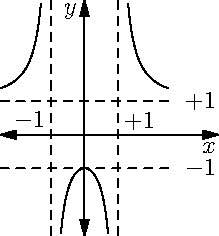
\includegraphics[width=0.75\linewidth]{graphics/algebra1.pdf}
\caption{$y=f(x)=\frac{x^2+1}{x^2-1}$}
\label{fig:algebra1}
\end{marginfigure}


And being asked to show
\begin{equation*}
    f(x+h)=\frac{x^2+1}{x^2-1}+ \frac{2h\cdot(2x+h)}{(x-1)(x+1)(x+h+1)(x+h-1)}
\end{equation*}
and
\begin{align*}
  |f(x)|<2 & \text{ if and only if } \\
           &  x \in (-\infty,-\sqrt{3})\cup(-\frac{1}{\sqrt{3}},+\frac{1}{\sqrt{3}})\cup(+\sqrt{3},+\infty)
\end{align*}
\begin{marginfigure}
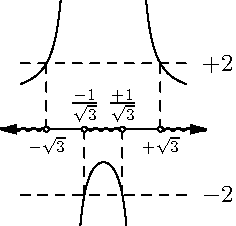
\includegraphics[width=0.75\linewidth]{graphics/algebra2.pdf}
\caption{Where $|f(x)|$ is less than $2$.}
\label{fig:algebra2}
\end{marginfigure}

should seem (at worst) tedious, but not mysterious.  Neither should the following:
\begin{equation*}
    2^{\log_3(x)}=x^{\log_2(3)} \,.
\end{equation*}
If these are mysterious to you, then you need to learn college algebra.
\section*{Trigonometry is helpful}

Additionally, it would be nice if you have some basic trigonometry, including measuring angles in radians, which is the only unit of angle we care about here.  For example,
\begin{marginfigure}
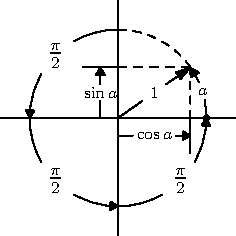
\includegraphics[width=0.75\linewidth]{graphics/unitcircle.pdf}
\caption{$x=\cos a$ and $y=\sin a$ defined on the unit circle in terms of the arc-length $a$ measured counter-clockwise from the $x$-axis.  This is what we mean when an angle is measured in radians, and why there are $2\pi$ radians in a circle.}
\label{fig:unitcircle}
\end{marginfigure}
\begin{align*}
    \cos a&=\pm\sqrt{1-(\sin a)^2}\,,\\
    \cos a&=
        \frac{1}{2}\text{ if and only if $x=3+2n$, for some integer $n$}\,,
\intertext{and}
    \sin(a+b)&=sin(a)cos(b)+cos(a)sin(b)\,,
\end{align*}
should at least be familiar to the point of looking something up to remember the details.

\section*{Reading Tips}
\begin{itemize}
\item Focus. The best environment for learning something mathematical is in a small group willing to help you work out a sudoku puzzle.  If you can't work out a sudoku puzzle in the place and with the people you study with, you will not learn mathematics.  You are also not a multi-tasker: you might multitask (usually poorly) on things you already understand; this is something you are trying to understand.
\item Drive, don't walk. Learning to use a computer algebra system can spare you from a lot of tedium compared to a crummy calculator.  Wolfram Alpha, Maxima, Maple, and Mathematica are all good choices.
\item Understand first. Proofs are less important than understanding.  If you are mostly interested in the applications of calculus, don't worry as much about understanding every proof.  Concentrate instead on understand why the facts that are shown make sense and how you mights use these facts.  If you are interested in mathematics itself, understanding the proofs are important, but pretty useless without an understanding of why they make sense and how to use them.
\end{itemize}
\section*{References}

Stitz Zeager -- [\url{www.stitz-zeager.com}]: algebra, trigonometry, and precalculus.

Boundless -- [\url{www.boundless.com}]: algebra and calculus.


\backmatter

\bibliography{bibliography} % Use the bibliography.bib file for the bibliography
\bibliographystyle{plainnat} % Use the plainnat style of referencing
\printindex % Print the index at the very end of the document

\end{document}
